\documentclass{article}
\usepackage[utf8]{inputenc}
\usepackage[T1]{fontenc}
\usepackage{pdfpages}
\usepackage{float}
\title{Wykrywacz Metali - Dokumentacja}
\author{
	Jakub Jaśków
	\and
	Justyna Ziemichód
}
\date{\today}

\begin{document}

\maketitle

\section{Funkcje Systemu}
\begin{itemize}
    \item Wykrywanie metali.
    \item Zmiana tonacji dźwięku.
    \item Czujnik odległości: Szacuje głębokość na której znajduje się wykryty obiekt.
    \item Wybór systemu powiadomiania: dźwięk, wibracje, LED
    \item Wybór czułości wykrywacza: większa czułość pozwala na wykrycie mniejszych lub słabiej przewodzących prąd obiektów. Skutkuje to jednak większą szansą odebrania zakłóceń.
    \item Wybór rodzaju metalu (dyskryminacja): Użytkownik może wybrać wykrywany rodzaj metalu (żelazo, złoto, srebro itp.).
\end{itemize}

\section{Realizacja Założeń}
	
- Wykrywanie metali: Cewka wykrywacza wytwarza fale elektromagnetyczne, które przenikają do gruntu, oraz dobera fale elektromagnetyczne wzbudzone w obiekcie, które odbierane są przez tą samą cewkę. Sygnał jest następnie przekazywane do mikrokontrolera, który zamienia go na dane, które są w odpowieni sposób przetwarzane. Jeżeli mikrokontroler wykryje, że fale elektromagnetyczne zostały zakłócone w sposób odpowiadający wybranemu rodzaju metalu, to poinformuje użytkownika w wybranych przez niego sposób.
\section{Środowisko i Ograniczenia}
System może być używany w różnych warunkach, zarówno wewnątrz pomieszczeń, jak i na zewnątrz. Jednakże jego skuteczność może być ograniczona przez warunki otoczenia, takie jak obecność innych źródeł metalu, zakłócenia elektromagnetyczne, mineralizacja gleby lub woda.

\section{Kategorie Użytkowników}
System wykrywacza metali może być wykorzystywany przez różne grupy użytkowników, w tym:
\begin{itemize}
    \item \textbf{Ochroniarze}: Używają wykrywacza do przeszukiwania osób i bagaży w celu wykrycia niepożądanych przedmiotów metalowych.
    \item \textbf{Poszukiwacze Skarbów}: Wykorzystują go do poszukiwania ukrytych obiektów metalowych, takich jak monety czy artefakty.
    \item \textbf{Geodeci}: Mogą używać go do wykrywania ukrytych rur lub kabli pod ziemią.
    \item\textbf{Śledczy}: Wykorzystują go do poszukiwania poszlak lub narzędzi zbrodni.
\end{itemize}

\section{Przypadki Użycia}

\begin{table}[htbp]
    \centering
    \caption{Włączenie wykrywacza}
    \label{tab:wlaczenie}
    \begin{tabular}{|l|l|}
    \hline
    \textbf{Nazwa PU} & Włączenie wykrywacza \\ \hline
    \textbf{Numer PU} & 001 \\ \hline
    \textbf{Priorytet} & Wysoki \\ \hline
    \textbf{Aktor podstawowy} & Użytkownik \\ \hline
    \textbf{Typ opisu} & Ogólny \\ \hline
    \textbf{Udziałowcy i cele} & Użytkownik: Włączenie wykrywacza w celu rozpoczęcia pracy. \\ \hline
    \textbf{Wyzwalacz} & Naciśnięcie przycisku zasilania na urządzeniu. \\ \hline
    \textbf{Typ wyzwalacza} & Zewnętrzny \\ \hline
    \textbf{Powiązania} & \\ \hline
    \textbf{Asocjacja} & PU 002. \\ \hline
    \textbf{Zawieranie} & PU 003, PU 004, PU 005, PU 006.\\ \hline
    \textbf{Rozszerzenie} & Brak.\\ \hline
    \textbf{Generalizacja} & Brak.\\ \hline
    \textbf{Zwykły przepływ zdarzeń} & \begin{tabular}[c]{@{}l@{}}1. Użytkownik wkłada akumulator na miejsce docelowe.\\2. Użytkownik przesuwa włącznik na pozycję ON.\\ 3. Wykrywacz uruchamia się.\end{tabular} \\ \hline
    \textbf{Przepływy poboczne} & Brak. \\ \hline
    \textbf{Przepływy alternatywne} & 1. Sprawdź czy akumulator jest naładowany. \\2.Sprawdź wyjście zasilania akumulatora i wejście zasilania wykrywacza. \\ 3. Skontaktuj się z producentem. \\ \hline
    \end{tabular}
\end{table}

\begin{table}[htbp]
    \centering
    \caption{Wyłączenie wykrywacza}
    \label{tab:wyłączenie}
    \begin{tabular}{|l|l|}
    \hline
    \textbf{Nazwa PU} & Wyłączenie wykrywacza \\ \hline
    \textbf{Numer PU} & 002 \\ \hline
    \textbf{Priorytet} & Wysoki \\ \hline
    \textbf{Aktor podstawowy} & Użytkownik \\ \hline
    \textbf{Typ opisu} & Ogólny \\ \hline
    \textbf{Udziałowcy i cele} & Użytkownik: Wyłączenie wykrywacza po zakończeniu pracy. \\ \hline
    \textbf{Wyzwalacz} & Naciśnięcie przycisku wyłączania na urządzeniu. \\ \hline
    \textbf{Typ wyzwalacza} & Zewnętrzny \\ \hline
    \textbf{Powiązania} & \\ \hline
    \textbf{Asocjacja} & PU002. \\ \hline
    \textbf{Zawieranie} & Brak.\\ \hline
    \textbf{Rozszerzenie} & Brak.\\ \hline
    \textbf{Generalizacja} & Brak.\\ \hline
    \textbf{Zwykły przepływ zdarzeń} & \begin{tabular}[c]{@{}l@{}}1. Użytkownik przesuwa włącznik na pozycję OFF.\\ 2. Wykrywacz zostaje wyłączony.\\ 3. Użytkownik wyjmuje akumulator\end{tabular} \\ \hline
    \textbf{Przepływy poboczne} & Brak. \\ \hline
    \textbf{Przepływy alternatywne} & 1. Wyjmij i włóż ponownie akumulator.\\ 2.Sprawdź czy incydent się powtarza. \\ 3. Jeżeli tak - skontatkuj się z producentem. \\ \hline
    \end{tabular}
\end{table}


\begin{table}[htbp]
    \centering
    \caption{Przejście do menu ustawień}
    \label{tab:menu-główne}
    \begin{tabular}{|l|l|}
    \hline
    \textbf{Nazwa PU} & Przejście do menu ustawień\\ \hline
    \textbf{Numer PU} & 006 \\ \hline
    \textbf{Priorytet} & Średni \\ \hline
    \textbf{Aktor podstawowy} & Użytkownik \\ \hline
    \textbf{Typ opisu} & Ogólny \\ \hline
    \textbf{Udziałowcy i cele} & Użytkownik: Przejście do menu ustawień. \\ \hline
    \textbf{Wyzwalacz} & Naciśnięcie przycisku USTAWIENIA na wyświetlaczu. \\ \hline
    \textbf{Typ wyzwalacza} & Zewnętrzny \\ \hline
    \textbf{Powiązania}& \\ \hline
    \textbf{Asocjacja} & PU 002. \\ \hline	
    \textbf{Zawieranie} & PU 003, PU 004, PU 005, PU 007.\\ \hline
    \textbf{Rozszerzenie} & PU 001.\\ \hline
    \textbf{Generalizacja} & Brak.\\ \hline
    \textbf{Zwykły przepływ zdarzeń} & 1. Użytkownik naciska przycisk USTAWIENIA na wyświetlaczu. \\2. Wyświetlacz zaczyna wyświetlać menu ustawień. \\ \hline
    \textbf{Przepływy poboczne} & Brak. \\ \hline
    \textbf{Przepływy alternatywne} & 1. Wyłącz urządzenie. \\ 2. Wyjmij i włóż ponownie akumulator. \\ 3. Włacz urządzenie.\\ 4.Sprawdź czy incydent się powtarza. \\ 5. Jeżeli tak - skontatkuj się z producentem. \\ \hline
    \end{tabular}
\end{table}


\begin{table}[htbp]
    \centering
    \caption{Zmiana sposobu sygnalizacji wykrycia metalu}
    \label{tab:zmiana-sygnalizacji}
    \begin{tabular}{|l|l|}
    \hline
    \textbf{Nazwa PU} & Zmiana sposobu sygnalizacji wykrycia metalu\\ \hline
    \textbf{Numer PU} & 003 \\ \hline
    \textbf{Priorytet} & Średni \\ \hline
    \textbf{Aktor podstawowy} & Użytkownik \\ \hline
    \textbf{Typ opisu} & Ogólny \\ \hline
    \textbf{Udziałowcy i cele} & Użytkownik: Zmiana sposobu sygnalizacji wykrycia metalu na wybrany przez użytkownika. \\ \hline
    \textbf{Wyzwalacz} & Wybór nowego sposobu sygnalizacji w menu ustawień. \\ \hline
    \textbf{Typ wyzwalacza} & Zewnętrzny \\ \hline
    \textbf{Powiązania}& \\ \hline
    \textbf{Asocjacja} & PU 006, PU 007, PU 008.\\ \hline
    \textbf{Zawieranie} & Brak.\\ \hline
    \textbf{Rozszerzenie} & PU 006.\\ \hline
    \textbf{Generalizacja} & Brak.\\ \hline    
    \textbf{Zwykły przepływ zdarzeń} & \begin{tabular}[c]{@{}l@{}}1. Użytkownik otwiera menu ustawień na wykrywaczu.\\ 2. Wybiera opcję zmiany sposobu sygnalizacji wykrycia metalu.\\ 3. Wybiera preferowany sposób sygnalizacji (np. dźwięk, wibracje, LED). \\ 4. Wyświetlany jest komunikat o tym czy zapisać ustawienia. \\5. Użytkownik naciska przycisk TAK\end{tabular} \\ \hline
    \textbf{Przepływy poboczne} & Brak. \\ \hline
    \textbf{Przepływy alternatywne} & 1. Wyłącz urządzenie. \\ 2. Wyjmij i włóż ponownie akumulator. \\ 3. Włacz urządzenie.\\ 4.Sprawdź czy incydent się powtarza. \\ 5. Jeżeli tak - skontatkuj się z producentem. \\ \hline
    \end{tabular}
\end{table}

\begin{table}[htbp]
    \centering
    \caption{Zmiana dyskryminacji}
    \label{tab:zmiana-dyskryminacji}
    \begin{tabular}{|l|l|}
    \hline
    \textbf{Nazwa PU} & Zmiana dyskryminacji \\ \hline
    \textbf{Numer PU} & 004 \\ \hline
    \textbf{Priorytet} & Średni \\ \hline
    \textbf{Aktor podstawowy} & Użytkownik \\ \hline
    \textbf{Typ opisu} & Szczegółowy \\ \hline
    \textbf{Udziałowcy i cele} & Użytkownik: Zmiana poziomu dyskryminacji, czyli rodzaju metalu, który ma być wykrywany. \\ \hline
    \textbf{Wyzwalacz} & Wybór nowego poziomu dyskryminacji w menu ustawień. \\ \hline
    \textbf{Powiązania} & \\ \hline
    \textbf{Asocjacja} & PU 006, PU 007, PU 008.\\ \hline
    \textbf{Zawieranie} & Brak.\\ \hline
    \textbf{Rozszerzenie} & PU 006.\\ \hline
    \textbf{Generalizacja} & Brak.\\ \hline
    \textbf{Typ wyzwalacza} & Zewnętrzny \\ \hline
    \textbf{Zwykły przepływ zdarzeń} & \begin{tabular}[c]{@{}l@{}}1. Użytkownik otwiera menu ustawień na wykrywaczu.\\ 2. Wybiera opcję zmiany poziomu dyskryminacji lub rodzaju metalu.\\ 3. Wybiera preferowany poziom dyskryminacji lub rodzaj metalu.\\ 4. Wyświetlany jest komunikat o tym czy zapisać ustawienia. \\5. Użytkownik naciska przycisk TAK\\ \end{tabular} \\ \hline
    \textbf{Przepływy poboczne} & Brak. \\ \hline
    \textbf{Przepływy alternatywne} & 1. Wyłącz urządzenie. \\ 2. Wyjmij i włóż ponownie akumulator. \\ 3. Włacz urządzenie.\\ 4.Sprawdź czy incydent się powtarza. \\ 5. Jeżeli tak - skontatkuj się z producentem. \\ \hline
    \end{tabular}
\end{table}

\begin{table}[htbp]
    \centering
    \caption{Zmiana czułości wykrywacza}
    \label{tab:zmiana-czulosci}
    \begin{tabular}{|l|l|}
    \hline
    \textbf{Nazwa PU} & Zmiana czułości \\ \hline
    \textbf{Numer PU} & 005 \\ \hline
    \textbf{Priorytet} & Średni \\ \hline
    \textbf{Aktor podstawowy} & Użytkownik \\ \hline
    \textbf{Typ opisu} & Ogólny \\ \hline
    \textbf{Udziałowcy i cele} & Użytkownik: Zmiana poziomu czułości wykrywacza, czyli jego zdolności do wykrywania mniejszych lub słabiej przewodzących metalowych obiektów. \\ \hline
    \textbf{Wyzwalacz} & Wybór nowego poziomu czułości w interfejsie użytkownika. \\ \hline
    \textbf{Powiązania} & \\ \hline
    \textbf{Asocjacja} & PU 006, PU 007, PU 008\\ \hline
    \textbf{Zawieranie} & Brak.\\ \hline
    \textbf{Rozszerzenie} & PU 006.\\ \hline
    \textbf{Generalizacja} & Brak.\\ \hline
    \textbf{Typ wyzwalacza} & Zewnętrzny \\ \hline
    \textbf{Zwykły przepływ zdarzeń} & \begin{tabular}[c]{@{}l@{}}1. Użytkownik otwiera menu ustawień na wykrywaczu.\\ 2. Wybiera opcję zmiany poziomu czułości.\\ 3. Wybiera preferowany poziom czułości.\\ 4. Wyświetlany jest komunikat o tym czy zapisać ustawienia \\5. Użytkownik naciska przycisk TAK\end{tabular} \\ \hline
    \textbf{Przepływy poboczne} & Brak. \\ \hline
    \textbf{Przepływy alternatywne} & 1. Wyłącz urządzenie. \\ 2. Wyjmij i włóż ponownie akumulator. \\ 3. Włacz urządzenie.\\ 4.Sprawdź czy incydent się powtarza. \\ 5. Jeżeli tak - skontatkuj się z producentem. \\ \hline
    \end{tabular}
\end{table}


\begin{table}[htbp]
    \centering
    \caption{Akceptacja zmain w ustawieniach}
    \label{tab:akceptacja-zmian}
    \begin{tabular}{|l|l|}
    \hline
    \textbf{Nazwa PU} & Akceptacja zmain w ustawieniach\\ \hline
    \textbf{Numer PU} & 007 \\ \hline
    \textbf{Priorytet} & Wysoki \\ \hline
    \textbf{Aktor podstawowy} & Użytkownik \\ \hline
    \textbf{Typ opisu} & Ogólny \\ \hline
    \textbf{Udziałowcy i cele} & Użytkownik: Akceptacja wprowadzonych zmian w ustawieniach. \\ \hline
    \textbf{Wyzwalacz} & Wprowadzenie zmian w ustawieniach i naciśnięcie przycisku ZAPISZ ZMIANY. \\ \hline
    \textbf{Powiązania} &\\ \hline
    \textbf{Asocjacja} & PU 003, PU 004, PU 005. \\ \hline
    \textbf{Zawieranie} & Brak.\\ \hline
    \textbf{Rozszerzenie} & PU 003, PU 004, PU 005.\\ \hline
    \textbf{Generalizacja} & Brak.\\ \hline
    \textbf{Typ wyzwalacza} & Zewnętrzny \\ \hline
    \textbf{Zwykły przepływ zdarzeń} & \begin{tabular}[c]{@{}l@{}}\\ 1. Wyświetlany jest komunikat o tym czy zapisać ustawienia \\2. Użytkownik naciska przycisk TAK\\3. Zmiany zostają wprowadzone oraz zapisane do pamięci urządzenia.\\4. Następuje powrót do menu ustawień.\end{tabular} \\ \hline
    \textbf{Przepływy poboczne} & Brak. \\ \hline
    \textbf{Przepływy alternatywne} & 1. Wyłącz urządzenie. \\ 2. Wyjmij i włóż ponownie akumulator. \\ 3. Włacz urządzenie.\\ 4.Sprawdź czy incydent się powtarza. \\ 5. Jeżeli tak - skontatkuj się z producentem. \\ \hline
    \end{tabular}
\end{table}


\begin{table}[htbp]
    \centering
    \caption{Anulowanie zmian ustawień}
    \label{tab:anulowanie-zmian}
    \begin{tabular}{|l|l|}
    \hline
    \textbf{Nazwa PU} & Anulowanie zmain w ustawieniach\\ \hline
    \textbf{Numer PU} & 008 \\ \hline
    \textbf{Priorytet} & Średni \\ \hline
    \textbf{Aktor podstawowy} & Użytkownik \\ \hline
    \textbf{Typ opisu} & Ogólny \\ \hline
    \textbf{Udziałowcy i cele} & Użytkownik: Anulowanie zmian wprowadzonych w ustawieniach. \\ \hline
    \textbf{Wyzwalacz} & Wprowadzenie zmian w ustawieniach i naciśnięcie przycisku ANULUJ. \\ \hline
    \textbf{Powiązania} & \\ \hline
    \textbf{Asocjacja} & PU 003, PU 004, PU 005. \\ \hline
    \textbf{Zawieranie} & Brak.\\ \hline
    \textbf{Rozszerzenie} & PU 003, PU 004, PU 005.\\ \hline
    \textbf{Generalizacja} & Brak.\\ \hline
    \textbf{Typ wyzwalacza} & Zewnętrzny \\ \hline
    \textbf{Zwykły przepływ zdarzeń} & \begin{tabular}[c]{@{}l@{}}1. Wyświetlany jest komunikat o tym czy zapisać ustawienia \\2. Użytkownik naciska przycisk ANULUJ\\3. Następuje powrót do menu ustawień.\end{tabular} \\ \hline
    \textbf{Przepływy poboczne} & Brak. \\ \hline
    \textbf{Przepływy alternatywne} & 1. Wyłącz urządzenie. \\ 2. Wyjmij i włóż ponownie akumulator. \\ 3. Włacz urządzenie.\\ 4.Sprawdź czy incydent się powtarza. \\ 5. Jeżeli tak - skontatkuj się z producentem. \\ \hline
    \end{tabular}
\end{table}

\begin{table}[htbp]
    \centering
    \caption{Powrót do ustawień fabrycznych}
    \label{tab:powrot-do-ustawien-fabrycznych}
    \begin{tabular}{|l|l|}
    \hline
    \textbf{Nazwa PU} & Powrót do ustawień fabrycznych\\ \hline
    \textbf{Numer PU} & 009 \\ \hline
    \textbf{Priorytet} & Średni \\ \hline
    \textbf{Aktor podstawowy} & Użytkownik \\ \hline
    \textbf{Typ opisu} & Ogólny \\ \hline
    \textbf{Udziałowcy i cele} & Użytkownik: Powrót do ustawień fabrycznych. \\ \hline
    \textbf{Wyzwalacz} & Naciśnięcie przycisku USTAWIENIA FABRYCZNE w menu ustawień. \\ \hline
        \textbf{Powiązania} & Asocjacja: Powiązane z PU 001 (Włączenie wykrywacza) - przeciwna operacja. \\ \hline
    \textbf{Powiązania} & \\ \hline
    \textbf{Asocjacja} & PU 006, PU 007, PU 008\\ \hline
    \textbf{Zawieranie} & Brak.\\ \hline
    \textbf{Rozszerzenie} & PU 006.\\ \hline
    \textbf{Generalizacja} & Brak.\\ \hline
    \textbf{Typ wyzwalacza} & Zewnętrzny \\ \hline
    \textbf{Zwykły przepływ zdarzeń} & \begin{tabular}[c]{@{}l@{}}\\ 1. Wyświetlany jest komunikat o tym czy na pewno przywrócić wszystkie ustawienia do ustawień fabrycznych\\2. Użytkownik naciska przycisk TAK\\3. Zmiany zostają zresetowane do ustawień fabrycznych.\\4. Następuje powrót do menu ustawień.\end{tabular} \\ \hline
    \textbf{Przepływy poboczne} & Brak. \\ \hline
    \textbf{Przepływy alternatywne} & 1. Wyłącz urządzenie. \\ 2. Wyjmij i włóż ponownie akumulator. \\ 3. Włacz urządzenie.\\ 4.Sprawdź czy incydent się powtarza. \\ 5. Jeżeli tak - skontatkuj się z producentem. \\ \hline
    \end{tabular}
\end{table}

\clearpage
\centering
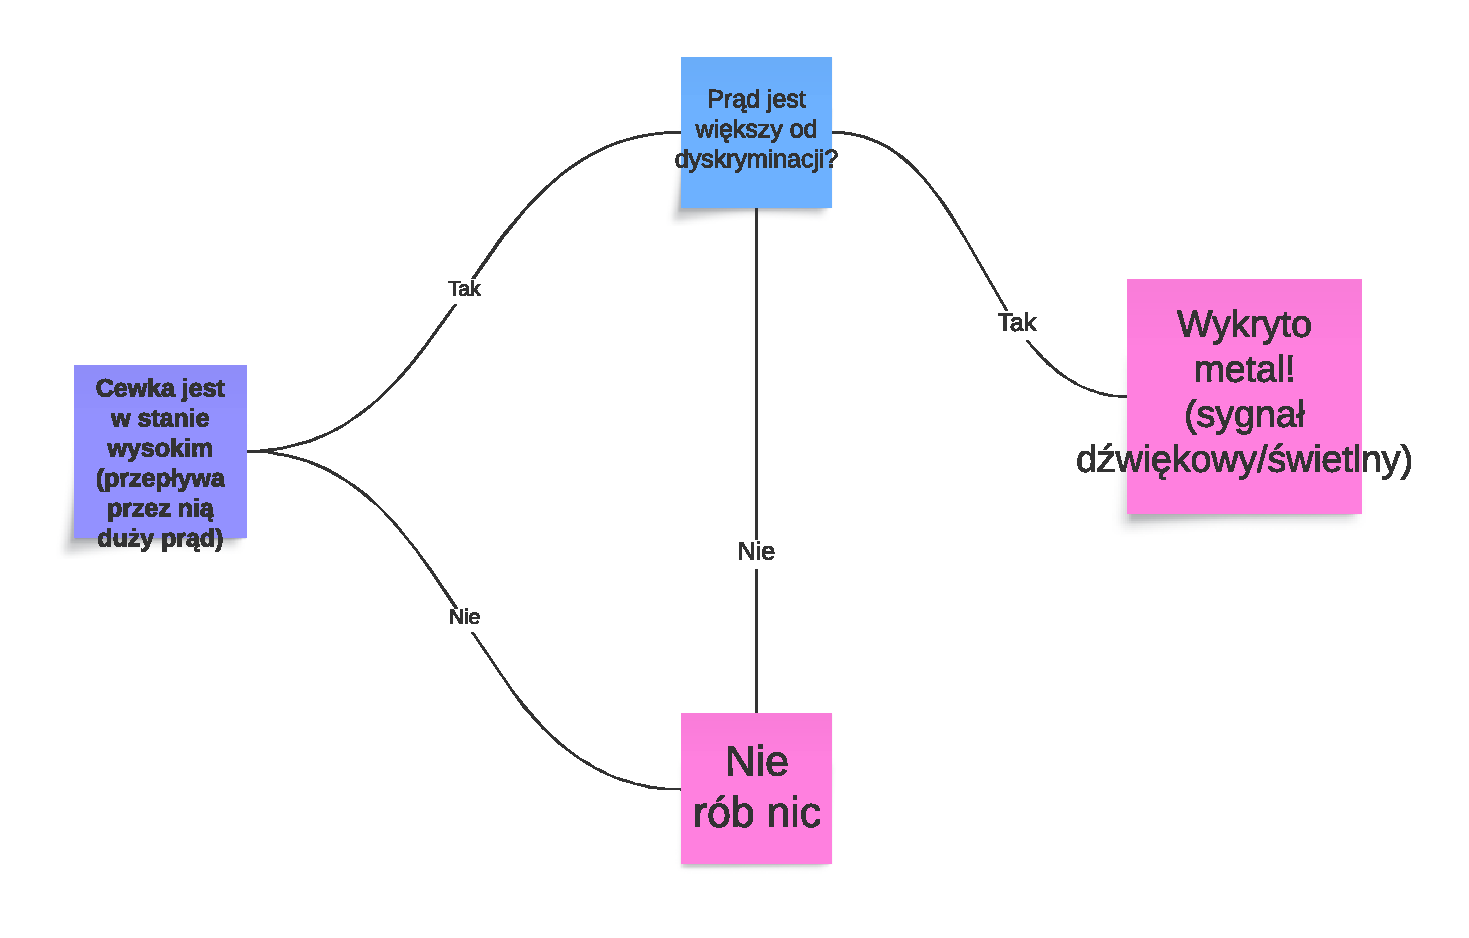
\includepdf[pages=-, pagecommand=\section{Diagram decyzyjny wykrywacza metalu}]{decision_tree.pdf}
\clearpage



\end{document}
